\documentclass{article}
\title{\LaTeX Math notes}
\author{Samuel Hautamäki}
\date{th of April 2025}
\usepackage{mathtools,amssymb,amsthm,gensymb,textcomp}
\usepackage{graphicx}
\graphicspath{ {./images/} }
\begin{document}
  \maketitle
   
  \section{Product rule}
  HL p 688\\
  If event A and B are independent then.\\
  $P(A and B)=P(A\cap B)=P(A)\cdot P(B)$\\
  Example May 2012/5 paper 1.\\
  P(2 white balls)=P(1st ball white and 2nd)\\
  $=P(1st is white)\cdot P(2nd is white)$\\
  $=\frac{3}{7}\cdot(\frac{2}{6})=\frac{3}{7}\cdot\frac{1}{3}=\frac{1}{7}$\\
  c) given that both are white, find the probability that they were chosen at bag A.\\
  Bag A is chosen if die gives 1 or 2, otherwise they are chosen from bag B.\\
  $P(bag A in condition 2 white)$\\
  $=\frac{P(bag A and 2 white)}{P(2 white)}=\frac{\frac{2}{6}\cdot\frac{1}{7}}{\frac{2}{6}\cdot\frac{1}{7}+\frac{4}{6}\cdot(\frac{4}{7}\cdot(\frac{3}{6}))}$\\
  $=\frac{1}{5}$\\
  for non-independent events\\
  $P(A\cap B)=P(A)=\cdot P(B|A)$\\
  $=P(B\cap A)=P(B)\cdot P(A|B)$\\
  where | means 'in condition that'\\
  Example 2.\\
  Find the probability of 2 hearts drawn from pack of playing cards.\\
  (without replacement)\\
  $P(1st is hearts and 2nd)=P(1st heart)\cdot P(2nd is heart| 1st was heart)$\\
  $=\frac{13}{52}\cdot(\frac{12}{51})=\frac{1}{4}\cdot\frac{4\cdot 3}{17\cdot 3}$\\
  HL p 692 ex 11B\\
  1. \\
  a) independent, because it doesn't matter what coin is, the prob of two sixes is same.\\
  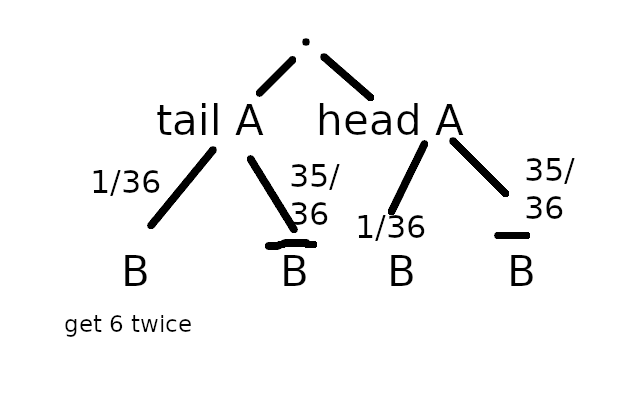
\includegraphics{23-4-11b-1-a}
  b) they are independent.\\
  2. \\
  b) i) $P(atleast one student went ziplining)=\frac{32}{50}=\frac{16}{25}$\\
  ii) $P(a student went orieenting given that thwy ent ziplining)=P(orienting | zip lining)=\frac{P(orienting and ziplining)}{P(zip lning)}=\frac{12/50}{16/25}=\frac{3}{8}$\\
  iii) P(orienting)=$\frac{26}{50}=\frac{13}{25}$\\
  iv) ziplining|orienting $\frac{P(zip linning and orienting)}{P(orienting)}=\frac{12/50}{13/25}=\frac{6}{13}$\\
  


\end{document}
